% TODO:

% Write ``Liquid-vapor interface'' section A.

% Look up question-mark references (citations).

\documentclass[letterpaper,twocolumn,amsmath,amssymb,prb]{revtex4-1}
\usepackage{graphicx}% Include figure files
\usepackage{dcolumn}% Align table columns on decimal point
\usepackage{bm}% bold math
\usepackage{color}

\newcommand{\red}[1]{{\bf \color{red} #1}}
\newcommand{\blue}[1]{{\bf \color{blue} #1}}
\newcommand{\green}[1]{{\bf \color{green} #1}}
\newcommand{\rr}{\textbf{r}}
\newcommand{\xx}{\textbf{x}}
\newcommand{\refnote}{\red{[ref]}}

\newcommand{\fixme}[1]{\red{[#1]}}

% needsworklater is used to annotate bits that need work, but that we
% can postpone for a while.
\newcommand{\needsworklater}[1]{\emph{[#1]}}
% needsworknow is intended to prioritize stuff that needs fixing.
\newcommand{\needsworknow}[1]{\textcolor{red}{[\emph{#1}]}}

\begin{document}
\title{A Fundamental Measure Theory Functional for Hard-Sphere Contact Densities}

\author{David Roundy}
\affiliation{Department of Physics, Oregon State University, Corvallis, OR 97331}

%%%%%%%%%%%%%%%%%%%%%%%%%%%%%%%%%%%%%%%%%%%%%%%%%%%%%%%%%%%%
\begin{abstract}
\needsworklater{ We develop a functional based on FMT~\cite{roth2002whitebear}
 to ... for SAFT}
\end{abstract}

\maketitle

%%%%%%%%%%%%%%%%%%%%%%%%%%%%%%%%%%%%%%%%%%%%%%%%%%%%%%%%%%%%
\section{Introduction}


\begin{figure}
\includegraphics[width=5cm]{figs/gHS-vs-n}
\caption{A comparison of the various approximations to the contact
  density.}
\label{fig:gHS-vs-n}
\end{figure}

\begin{figure}
\includegraphics[width=5cm]{figs/free-energy}
\caption{A comparison of the various approximations to the free
  energy.  Note that the White Bear functional uses a modified form of
  the Carnahan equation of state.}
\label{fig:free-energy}
\end{figure}

The hard-sphere contact density---which we will define as the density
of hard spheres touching a given hard sphere---is important for the
association term in Statistical Associating Fluid Theory (SAFT).  For
a homogeneous hard-sphere fluid, the contact density---which is to
say, $n g_{HS}(\sigma)$---is easily computed from the
Carnahan-Starling equation of state
\begin{align}
  g_{HS}(\sigma) &= \frac{1}{1-\eta} + \cdots
\end{align}
The contact density may be easily computed from a knowledge of the
contact theorem, which states that the pressure on any hard surface is
given by
\begin{align}
  p &= k_BT n_\textit{contact}
\end{align}
Since we are interested in the contact density at the hard-sphere
surface, all we need compute is the pressure on that surface, and
we'll have our answer.  The pressure on a hard sphere can be readily
computed from the dependence of the free energy on hard sphere
radius.
\begin{align}
  A_{HS} &= Nk_BT \frac{4\eta - 3\eta^2}{(1-\eta)^2}
\end{align}
Since $\eta \equiv \frac{4\pi}{3} R^3$, we can work out that
\begin{align}
  \frac{dA_{HS}}{dR} &= \frac{dA_{HS}}{d\eta} \frac{d\eta}{dR} \\
  &= Nk_BT \left( \frac{4 - 6\eta}{(1-\eta)^2} + 2 \frac{4\eta - 3\eta^2}{(1-\eta)^3} \right) \frac{d\eta}{dR}
  \\
  &= Nk_BT \frac{4 - 4\eta - 6\eta + 6\eta^2 + 8\eta - 6\eta^2}{(1-\eta)^3} \frac{d\eta}{dR}
  \\
  &= Nk_BT \frac{4 - 2\eta}{(1-\eta)^3} \frac{d\eta}{dR}
  \\
  &= Nk_BT \frac{4 - 2\eta}{(1-\eta)^3} \frac{3 \eta}{R} \label{eq:dAhsdR}
\end{align}
This derivative gives us the force on \emph{all} the hard
spheres---since we're changing all their radii at once.  To compute
the pressure on the spheres, we just need to divide by the total area,
which means dividing by $N 4\pi (2R)^2$.  The area which is relevant
is the area over which the molecules can make contact.
\begin{align}
  p_{HS} &= \frac{1}{N 4\pi (2R)^2} \frac{dA_{HS}}{dR} \\
  &= \frac14 \frac{1}{N 4\pi R^2} Nk_BT \frac{4 - 2\eta}{(1-\eta)^3} \frac{3 \eta}{R} \\
  &= \frac{3}{4\pi R^3} \eta k_BT \frac{1 - \frac{\eta}2}{(1-\eta)^3} \\
  &= n k_BT \frac{1 - \frac{\eta}2}{(1-\eta)^3}
\end{align}
\begin{align}
  n_\textit{contact} &= n \frac{1 - \frac{\eta}2}{(1-\eta)^3} \\
  g_{HS}(\sigma) &= \frac{1 - \frac{\eta}2}{(1-\eta)^3}
\end{align}
As it turns out, this is the standard answer for the contact value of
the autocorrelation function! $\ddot\smile$

\section{Fundamental-Measure Theory}

We use the White Bear version of the Fundamental-Measure Theory~(FMT)
functional published in reference~\cite{roth2002whitebear}.  The FMT
functional describes the excess free energy of a hard-sphere fluid.
This particular FMT reduces to the Carnahan-Starling equation of state
for homogeneous systems.
\begin{equation}
A_\textit{HS}[n] = k_B T \int \left(\Phi_1(\xx) + \Phi_2(\xx) + \Phi_3(\xx)\right) d\xx \; ,
\end{equation}
with integrands
\begin{align}
\Phi_1 &= -n_0 \ln\left( 1 - n_3\right)\\
\Phi_2 &= \frac{n_1 n_2 - \mathbf{n}_{V1} \cdot\mathbf{n}_{V2}}{1-n_3} \\
\Phi_3 &= (n_2^3 - 3 n_2 \mathbf{n}_{V2} \cdot \mathbf{n}_{V2}) \frac{
  n_3 + (1-n_3)^2 \ln(1-n_3)
}{
  36\pi n_3^2\left( 1 - n_3 \right)^2
} ,
\end{align}
using the weighted densities
\begin{align}
  n_3(\xx) &= \int n(\xx') \Theta(\left|\xx - \xx'\right| - R) d\xx' \\
  n_2(\xx) &= \int n(\xx') \delta(\left|\xx - \xx'\right| - R) d\xx'
\end{align}
\begin{align}
  \mathbf{n}_{V2} &= \mathbf{\nabla} n_3 , \quad
  \mathbf{n}_{V1} = \frac{\mathbf{n}_{V2}}{4\pi R} \\
  n_1 &= \frac{n_2}{4\pi R} , \quad
  n_0 = \frac{n_2}{4\pi R^2}
\end{align}

\begin{widetext}

\section{Mean Contact density}

One reasonably simple question to ask is what the \emph{mean} contact
density of an inhomogeneous system is.  This comes down to simply
reproducing the derivation for a homogeneous system using the
FMT functional.
\begin{align}
  p_{HS} &= \frac{1}{N 4\pi (2R)^2} \frac{dA_{HS}}{dR}
\end{align}
So to compute this we need
\begin{align}
  \frac{d A_{HS}}{d R} &=
  \frac{\partial A_{HS}}{\partial R} \\
  &+
  \int \left(
  \frac{\delta A_{HS}}{\delta n_3(\mathbf{r}')}
  \frac{d n_3(\mathbf{r}')}{d R}
  +
  \frac{\delta A_{HS}}{\delta n_2(\mathbf{r}')}
  \frac{d n_2(\mathbf{r}')}{d R}
  + \cdots
  \right) d\mathbf{r}'
\end{align}

\begin{align}
  \frac{dn_3(\mathbf{r})}{dR} &= n_2(\mathbf{r})\\
  \frac{dn_2(\mathbf{r})}{dR} &= \int n(\mathbf{r}+\mathbf{r}')
  \delta'(|\mathbf{r'}| - R)\mathbf{dr}'\\
  &= \int n(\mathbf{r}+\mathbf{r}')
  \delta'(r' - R) d\Omega' r'^2 dr'\\
  &= \int 
  \delta(r' - R) d\Omega' \left(\frac{dn(\mathbf{r}+\mathbf{r}')}{dr'}r'^2 + 2n(\mathbf{r}+\mathbf{r}')r' \right) dr'\\
  &= \frac1{R} \int 
  \delta(|\mathbf{r}'| - R)
  \left(\mathbf{r}'\cdot \nabla n(\mathbf{r}+\mathbf{r}') +
  2n(\mathbf{r}+\mathbf{r}') \right) \mathbf{dr}' \\
  &= \frac{2}{R}n_2(\mathbf{r}) + \frac{1}{R} \int 
  \delta(|\mathbf{r}'| - R)\mathbf{r}'\cdot \nabla n(\mathbf{r}+\mathbf{r}') \mathbf{dr}' \\
  \frac{dn_0(\mathbf{r})}{dR} &= \frac{1}{R} \int 
  \delta(|\mathbf{r}'| - R)\mathbf{r}'\cdot \nabla n(\mathbf{r}+\mathbf{r}') \mathbf{dr}' \\
  \frac{dn_1(\mathbf{r})}{dR} &=
    \frac1{4\pi R}\frac{dn_2(\mathbf{r})}{dR} - n_0(\mathbf{r}) \\
    &= n_0(\mathbf{r}) + \frac{1}{4\pi R^2} \int 
    \delta(|\mathbf{r}'| - R)\mathbf{r}'\cdot \nabla n(\mathbf{r}+\mathbf{r}') \mathbf{dr}' \\
  \frac{d\mathbf{n}_{V2}}{dR} &= \nabla n_2
\end{align}

The total force due to $\Phi_1$ is actually very easy to work out:
\begin{align}
  \frac{d A_{HS}^{(1)}}{d R} &=
  \int \mathbf{dr}' \left(\frac{n_0n_2}{1-n_3} - \frac{dn_0(\mathbf{r})}{dR}\ln(1-n_3) \right)
\end{align}
where you can see that $\frac{dn_0(\mathbf{r})}{dR}$ is zero for a
homogeneous system, and small for reasonably smooth density
distributions.  The next term from $\Phi_2$ is as follows:
\begin{align}
  \frac{d A_{HS}^{(2)}}{d R} &=
  \int \mathbf{dr}' \left(
    \frac{n_1 n_2 - \mathbf{n}_{V1} \cdot\mathbf{n}_{V2}}{(1-n_3)^2}
    n_2
    - \frac{n_0n_2 - \mathbf{n}_{V0} \cdot\mathbf{n}_{V2} - 2 n_1
      \frac{dn_2}{dR} + 2 \mathbf{n}_{V1} \cdot \nabla n_2 \cdot
    }{1-n_3}
  \right) \\
  &= \int \mathbf{dr}' \left(
    \frac{n_1 n_2 - \mathbf{n}_{V1} \cdot\mathbf{n}_{V2}}{(1-n_3)^2}
    n_2
    - \frac{n_0n_2 - \mathbf{n}_{V0} \cdot\mathbf{n}_{V2}
      - 2 n_1 \left(\frac2{R}n_2 \frac{dn_0}{dR}\right)
      + 2 \mathbf{n}_{V1} \cdot \nabla n_2 \cdot }{1-n_3}
  \right) \\
  &= \int \mathbf{dr}' \left(
    \frac{n_1 n_2 - \mathbf{n}_{V1} \cdot\mathbf{n}_{V2}}{(1-n_3)^2}
    n_2
    - \frac{n_0n_2 - \mathbf{n}_{V0} \cdot\mathbf{n}_{V2}
      - 4 n_0n_2 - 2 n_1\frac{dn_0}{dR}
      + 2 \mathbf{n}_{V1} \cdot \nabla n_2 \cdot }{1-n_3}
  \right) \\
  &= \int \mathbf{dr}' \left(
    \frac{n_1 n_2 - \mathbf{n}_{V1} \cdot\mathbf{n}_{V2}}{(1-n_3)^2}
    n_2
    + \frac{3n_0n_2 + \mathbf{n}_{V0} \cdot\mathbf{n}_{V2}
      + 2 n_1\frac{dn_0}{dR}
      - 2 \mathbf{n}_{V1} \cdot \nabla n_2 \cdot }{1-n_3}
  \right)
\end{align}

And the last term looks like this.  I should perhaps note that this
term should be replaced by a tensor version if want to examine
seriously localized density distributions.
\begin{align}
  A_{HS}^{(3)} &=
  \int \mathbf{dr}'\left(
     (n_2^3 - 3n_2\mathbf{n}_{V2} \cdot \mathbf{n}_{V2})
     \frac{
       n_3 + (1-n_3)^2 \ln(1-n_3)
     }{
       36\pi n_3^2\left( 1 - n_3 \right)^2
     }
  \right) \\
  \frac{d A_{HS}^{(3)}}{d R} &=
  \int \mathbf{dr}'
     \left[
       3(n_2^2 - \mathbf{n}_{V2} \cdot \mathbf{n}_{V2})
       \left(\frac2{R}n_2 + \frac{dn_0}{dR}\right)
       - 6n_2 \mathbf{n}_{V2} \cdot \nabla n_2
     \right]
     \frac{
       n_3 + (1-n_3)^2 \ln(1-n_3)
     }{
       36\pi n_3^2\left( 1 - n_3 \right)^2
     }
   \\
  &+
     (n_2^3 - 3n_2\mathbf{n}_{V2} \cdot \mathbf{n}_{V2}) n_2
     \frac{
       (1 - 2(1-n_3)\ln(1-n_3) - (1-n_3))n_3^2( 1 - n_3)^2
       -
       (n_3 + (1-n_3)^2 \ln(1-n_3))(-2 n_3^2( 1 - n_3) + 2n_3(1-n_3)^2)
     }{
       36\pi (n_3^2\left( 1 - n_3 \right)^2)^2
     }
     \\
     &=
     \int \mathbf{dr}'
     \left[
       (n_1n_2 - \mathbf{n}_{V1} \cdot \mathbf{n}_{V2})
       \left(2n_2 + \frac{1}{4\pi}\frac{dn_0}{dR}\right)
       - \frac{1}{2\pi}n_2 \mathbf{n}_{V2} \cdot \nabla n_2
     \right]
     \frac{
       n_3 + (1-n_3)^2 \ln(1-n_3)
     }{
       3 n_3^2\left( 1 - n_3 \right)^2
     }
   \\
  &+
     \frac{n_2(n_2^3 - 3n_2\mathbf{n}_{V2} \cdot \mathbf{n}_{V2})}{36\pi}
   \left( \frac{1}{(1-n_3)^2} + 2 \frac{\ln(1-n_3)}{n_3^2(1-n_3)} \right)
\end{align}

\begin{align}
  \frac{d A_{HS}}{d R} &=
  \int \mathbf{dr}' \left(
    -\frac{n_0n_2}{1-n_3} - \frac{dn_0(\mathbf{r})}{dR}\ln(1-n_3)
    + \cdots
  \right)
\end{align}

\section{Contact density at a given hard sphere}

When we consider an inhomogeneous system, we may ask for \emph{which}
sphere we are interested in computing the contact density.  One way to
answer this is to specify a sphere at a fixed position $\mathbf{r}$.
By making the hard-sphere radius dependent on position, we can compute
the pressure on the hard spheres located at $\mathbf{r}$.
\begin{align}
  p_{HS}(\mathbf{r}) &= \frac{1}{4\pi (2R)^2} \frac{\delta A_{HS}}{\delta R(\mathbf{r})}
\end{align}
So to compute this we need
\begin{align}
  \frac{\delta A_{HS}}{\delta R(\mathbf{r})} &=
  \int \left(
  \frac{\delta A_{HS}}{\delta n_3(\mathbf{r}')}
  \frac{\delta n_3(\mathbf{r}')}{\delta R(\mathbf{r})}
  +
  \frac{\delta A_{HS}}{\delta n_2(\mathbf{r}')}
  \frac{\delta n_2(\mathbf{r}')}{\delta R(\mathbf{r})}
  + \cdots
  \right) d\mathbf{r}'
\end{align}
There are \emph{many} such terms, and this could get expensive.

  First, let's rewrite the free energy in terms of a smaller set of
  weighted densities:
  \begin{align}
    A_{HS} &= \int \left\{
      -n_0 \ln\left( 1 - n_3\right)
      + \frac{n_1 n_2 - \mathbf{n}_{V1} \cdot\mathbf{n}_{V2}}{1-n_3}
      + (n_2^3 - 3 n_2 \mathbf{n}_{V2} \cdot \mathbf{n}_{V2}) \frac{
        n_3 + (1-n_3)^2 \ln(1-n_3)
      }{
        36\pi n_3^2(1-n_3)^2
      }
    \right\}
    \\
    &= \int \left\{
      -\frac{n_2}{4\pi R^2} \ln\left( 1 - n_3\right)
      + \frac{1}{4\pi R} \frac{n_2^2 - \mathbf{n}_{V2} \cdot\mathbf{n}_{V2}}{1-n_3}
      + (n_2^3 - 3 n_2 \mathbf{n}_{V2} \cdot \mathbf{n}_{V2}) \frac{
        n_3 + (1-n_3)^2 \ln(1-n_3)
      }{
        36\pi n_3^2(1-n_3)^2
      }
    \right\}
\end{align}

\begin{align}
    \frac{\delta A_{HS}}{\delta n_3(\mathbf{r}')} &=
    -\frac{n_0(\mathbf{r}')}{1 - n_3(\mathbf{r}')}
    + \frac{n_1n_2 - \mathbf{n}_{V1}\cdot\mathbf{n}_{V2}}{(1 -
      n_3(\mathbf{r}'))^2}
    + \frac{n_2^3 -
      3n_2\mathbf{n}_{V2}\cdot\mathbf{n}_{V2}}{36\pi}\left(
      \frac{1}{(1-n_3)^2} + 2\frac{\ln(1-n_3)}{n_2^2(1-n_3)}
    \right)
    \\
    \frac{\delta A_{HS}}{\delta n_2(\mathbf{r}')} &=
    -\frac{1}{4\pi R^2} \ln\left( 1 - n_3\right)
    +  \frac{2n_1}{1-n_3}
    + 3(n_2^2 - \mathbf{n}_{V2}\cdot\mathbf{n}_{V2})\frac{n_3 +
      (1-n_3)^2\ln(1-n_3)}{
      36\pi n_3^2(1-n_3)^2
    }
    \\
    \frac{\delta A_{HS}}{\delta \mathbf{n}_{V2}(\mathbf{r}')} &=
    \frac{2\mathbf{n}_{V1}}{1-n_3}
    - 6 n_2 \mathbf{n}_{V2} \frac{n_3 +
      (1-n_3)^2\ln(1-n_3)}{
      36\pi n_3^2(1-n_3)^2
    }    \\
    \frac{\delta A_{HS}}{\delta R(\mathbf{r}')} &=
    \frac{n_2}{2\pi R^3} \ln\left( 1 - n_3\right)
    - \frac1{R} \frac{n_1n_2 - \mathbf{n}_{V1} \cdot\mathbf{n}_{V2}}{1-n_3}
  \end{align}

\begin{align}
  \frac{\delta n_3(\mathbf{r}')}{\delta R(\mathbf{r})} &=
  n(\mathbf{r})\delta(|\mathbf{r}-\mathbf{r}'| - R) \\
  \frac{\delta n_2(\mathbf{r}')}{\delta R(\mathbf{r})} &=
  n(\mathbf{r}) \delta'(|\mathbf{r}-\mathbf{r}'| - R) \\
  \frac{\delta \mathbf{n}_{V2}(\mathbf{r}')}{\delta R(\mathbf{r})} &=
  -\frac{\delta}{\delta R(\mathbf{r})} \mathbf{\nabla}' n_3(\mathbf{r}')
  \\
  &= -\mathbf{\nabla}'
  \left(n(\mathbf{r})\delta(|\mathbf{r}-\mathbf{r}'| - R) \right)
\end{align}
These give us some basic tools with which to perform derivatives.

Finally, we get an answer like
\begin{align}
  \frac{\delta A_{HS}}{\delta R(\mathbf{r})} &=
  \int \mathbf{dr}' \left\{
  \left(
  \frac{n_0(\mathbf{r}')}{1 - n_3(\mathbf{r}')}
  + \frac{n_1n_2 - \mathbf{n}_{V1}\cdot\mathbf{n}_{V2}}{(1 -
    n_3(\mathbf{r}'))^2}
  + \frac{1}{4\pi}\frac{
    \frac13 n_2^3 - n_2 \mathbf{n}_{V2} \cdot \mathbf{n}_{V2}
  }{
    (1-n_3(\mathbf{r}'))^3
  }
  \right) n(\mathbf{r}') \delta(|\mathbf{r}-\mathbf{r}'| - R)
  + \cdots
  \right\}
\end{align}
This comes out to quite a mess.  It wouldn't be infeasible to compute
this, but it wouldn't be efficient or pretty either.

\begin{figure}
\includegraphics[width=5cm]{figs/n0}
\caption{Set of hard spheres that included in $n_0(\mathbf{r})$, which
  consist of those which just touch the point $\mathbf{r}$.}
\label{fig:n0}
\end{figure}

\section{Contact density at a given contact position}

Unfortunately, knowing the average contact density on each hard sphere
doesn't really give us what we want for SAFT.  The trouble is that in
order to work out the fraction of association sites occupied, we need
to know the contact density \emph{at the point of contact}.
Fortunately, we don't need to know the contact density for a
particular sphere at each point of contact.  Just as $n_0(\mathbf{r})$
gives us the density of spheres that are contacting point $\mathbf{r}$
(see Figure~\ref{fig:n0}), we can use similar reasoning to work out the
contact density for these spheres.

To find the contact density at a given point of contact, we can't
simply change the radius for spheres touching that point, since that
would give us the pressure averaged over the entire surface of those
spheres.  Instead, we'll have to imagine extending a patch of those
spheres which is located at the point of interest, as illustrated in
Figure~\ref{fig:contact}.

\begin{figure}
\includegraphics[width=5cm]{figs/contact}
\caption{Construction for finding the contact density at a given point
  of contact.  We envision a small area $dA$ of each sphere that touches
the point $\mathbf{r}$ extended by a distance $dR$.}
\label{fig:contact}
\end{figure}

So we need to find the small change in free energy that is caused by
these small changes in the shape and size of the hard spheres that are
in contact with this point.  In the following section, we will work
out the changes in the weighted densities at position $\mathbf{r}'$
when point of contact we are considering is $\mathbf{r}$.

The packing fraction $n_3$ is changed at the point where the sphere is
extended, since a few more spheres will overlap this point.
\begin{align}
  \Delta n_3(\mathbf{r}') &= n(\mathbf{r})\Delta A \Delta R
  \delta(|\mathbf{r}-\mathbf{r}'| - R)
\end{align}
The density $n_0$ is the average density, averaged over a spherical
shell.  As such, shifting the position of a shell just shifts which
location we are averaging over.
\begin{align}
  \Delta n_0(\mathbf{r}') &=
    \frac{\mathbf{r}-\mathbf{r}'}{|\mathbf{r}-\mathbf{r}'|}\cdot
      \mathbf{\nabla}n(\mathbf{r}) \Delta A \Delta R
    \delta(|\mathbf{r}-\mathbf{r}'|-R)
\end{align}
The change in $n_2$ comes from two terms: a change in the density value, as
we saw in $n_0$, and a change in the area of the segment.
\begin{align}
  \Delta n_2(\mathbf{r}') &=
  \left(n\left(\mathbf{r} + \Delta R
  \frac{\mathbf{r}-\mathbf{r}'}{|\mathbf{r}-\mathbf{r}'|}\right)\left(1+2\frac{\Delta
  R}{R}\right)- n(\mathbf{r})\right) \Delta A
  \delta(|\mathbf{r}-\mathbf{r}'|-R) \\
  &=
  \left(\frac{\mathbf{r}-\mathbf{r}'}{|\mathbf{r}-\mathbf{r}'|}\cdot
    \mathbf{\nabla}n(\mathbf{r}) + 2 \frac{n(\mathbf{r})}{R}
    \right) \Delta A \Delta R
  \delta(|\mathbf{r}-\mathbf{r}'|-R)
\end{align}
The vector density $\mathbf{n}_{V2}$ is similar to the density
$n_2$: both changes in the density value and changes in the surface
area play a role.
\begin{align}
  \Delta \mathbf{n}_{V2}(\mathbf{r}') &=
  \frac{\mathbf{r}-\mathbf{r}'}{|\mathbf{r}-\mathbf{r}'|}
  \left(n\left(\mathbf{r} + \Delta R
  \frac{\mathbf{r}-\mathbf{r}'}{|\mathbf{r}-\mathbf{r}'|}\right)\left(1+2\frac{\Delta
  R}{R}\right)- n(\mathbf{r})\right) \Delta A
  \delta(|\mathbf{r}-\mathbf{r}'|-R) \\
  &=
  \frac{\mathbf{r}-\mathbf{r}'}{|\mathbf{r}-\mathbf{r}'|}
  \left(\frac{\mathbf{r}-\mathbf{r}'}{|\mathbf{r}-\mathbf{r}'|}\cdot
    \mathbf{\nabla}n(\mathbf{r}) + 2 \frac{n(\mathbf{r})}{R}
    \right) \Delta A \Delta R
  \delta(|\mathbf{r}-\mathbf{r}'|-R) 
\end{align}
The density $n_1$ (and similarly $\mathbf{n}_{V1}$) can be roughly
interpreted as the density weighted by the area-averaged mean
curvature~\cite{oversteegen2005general, roth2010review}.  When we
extend the sphere at the contact point, we will introduce regions of
both positive and negative mean curvature.  In principle, we can do
this in such a way that the two portions cancel, and hence we will
assume that
\begin{align}
  \Delta n_1(\mathbf{r}') &= 0 \\
  \Delta \mathbf{n}_{V1}(\mathbf{r}') &= 0
\end{align}
In fact, the negative and positive portions are spatially separated,
so these terms should probably include a derivative term, which I
should work out.  Particularly as it may even happen to cancel a
different derivative term that we then won't have to drop!

We need to then find the change in Helmholtz free energy due to this
change at position $\mathbf{r}$:
\begin{align}
  \Delta A_{HS} &= \int \mathbf{dr}'
  \frac{\delta A_{HS}}{\delta n_3(\mathbf{r}')}\Delta n_3(\mathbf{r}')
  +
  \frac{\delta A_{HS}}{\delta n_2(\mathbf{r}')}\Delta n_2(\mathbf{r}')
  +
  \frac{\delta A_{HS}}{\delta \mathbf{n}_{V2}(\mathbf{r}')} \cdot \Delta \mathbf{n}_{V2}(\mathbf{r}')
\end{align}

\end{widetext}

%%%%%%%%%%%%%%%%%%%%%%%%%%%%%%%%%%%%%%%%%%%%%%%%%%%%%%%%%%%%
\section{Conclusion}
We get a nice spatial dependence for SAFT.

\begin{widetext}
  \appendix

  \section{Partial derivatives of the White Bear free energy functional}

  Here is the White Bear free energy functional for the hard-sphere
  fluid:~\cite{roth2002whitebear}
  \begin{align}
    \beta A_{HS} &= \int \left\{
    -n_0 \ln\left( 1 - n_3\right)
    + \frac{n_1 n_2 - \mathbf{n}_{V1} \cdot\mathbf{n}_{V2}}{1-n_3}
    + (n_2^3 - 3 n_2 \mathbf{n}_{V2} \cdot \mathbf{n}_{V2}) \frac{
      n_3 + (1-n_3)^2 \ln(1-n_3)
    }{
      36\pi n_3^2(1-n_3)^2
    }
    \right\}
\end{align}

\begin{align}
    \beta\frac{\delta A_{HS}}{\delta n_3(\mathbf{r}')} &=
    \frac{n_0(\mathbf{r}')}{1 - n_3(\mathbf{r}')}
    + \frac{n_1n_2 - \mathbf{n}_{V1}\cdot\mathbf{n}_{V2}}{(1 -
      n_3(\mathbf{r}'))^2}
    + \frac{n_2^3 -
      3n_2\mathbf{n}_{V2}\cdot\mathbf{n}_{V2}}{36\pi}
    %\left(
    %  \frac{1}{(1-n_3)^2} + 2\frac{\ln(1-n_3)}{n_2^2(1-n_3)}
    %\right)
    \\
    & \times \left(\frac{2}{n_3(1-n_3)^3} -\frac1{n_3^2(1-n_3)^2}  -
      \frac{1}{n_3^2(1-n_3)} - 2\frac{\ln(1-n_3)}{n_3^3}\right) \\
    \beta\frac{\partial A_{HS}}{\partial n_3}
    &\sim \frac{n}{1-\eta} + \frac{3n\eta}{(1-\eta)^2} +
      \frac{2n\eta}{(1-\eta)^3} -
      \frac{n}{(1-\eta)^2} -
      \frac{n}{1-\eta} -
      2n \frac{ \ln(1-\eta) }{ \eta } \\
    &= \frac{3n\eta}{(1-\eta)^2} +
      \frac{2n\eta}{(1-\eta)^3} -
      \frac{n}{(1-\eta)^2} -
      2n \frac{ \ln(1-\eta) }{ \eta } \\
    &= n\left(
      \frac{3\eta - 3 \eta^2}{(1-\eta)^3} +
      \frac{2\eta}{(1-\eta)^3} -
      \frac{1 - \eta}{(1-\eta)^3} -
      2 \frac{ \ln(1-\eta) }{ \eta }
      \right) \\
    &= n\left(
      \frac{6\eta - 3 \eta^2 - 1}{(1-\eta)^3} -
      2 \frac{ \ln(1-\eta) }{ \eta }
      \right)
\end{align}
\end{widetext}

\begin{align}
    \beta\frac{\delta A_{HS}}{\delta n_0(\mathbf{r}')} &= -\ln(1-n_3)
    \\
    \beta\frac{\delta A_{HS}}{\delta n_1(\mathbf{r}')} &= \frac{n_2}{1-n_3}
    \\
    \beta\frac{\partial A_{HS}}{\partial n_1}
    &\sim n \frac{4\pi R^2}{1-\eta}
\end{align}
\begin{align}
    \beta\frac{\delta A_{HS}}{\delta n_2(\mathbf{r}')} &=
      \frac{n_1}{1-n_3}
      + (n_2^2 - \mathbf{n}_{V2}\cdot\mathbf{n}_{V2})\frac{n_3 +
        (1-n_3)^2\ln(1-n_3)}{
        12\pi n_3^2(1-n_3)^2
      }
\end{align}
\begin{align}
    \beta\frac{\partial A_{HS}}{\partial n_2}
    &\sim n\frac{R}{1-\eta} +
    \frac{4\pi}{3} R^4 n^2 \frac{\eta + (1-\eta)^2\ln(1-\eta)}{\eta^2(1-\eta)^2}
    \\
    &= n\frac{R}{1-\eta} +
    \frac{R n}{(1-\eta)^2}
    + Rn \frac{\ln(1-\eta)}{\eta}
    \\
    &= nR\left( \frac{1 + \eta^2  - 2\eta}{(1-\eta)^3} +
      \frac{1 - \eta}{(1-\eta)^3}
    + \frac{\ln(1-\eta)}{\eta}
    \right)
    \\
    &= nR\left( \frac{2 + \eta^2  - 3\eta}{(1-\eta)^3}
    + \frac{\ln(1-\eta)}{\eta}
    \right)
\end{align}
\begin{align}
    \beta\frac{\delta A_{HS}}{\delta \mathbf{n}_{V1}(\mathbf{r}')} &=
      \frac{\mathbf{n}_{V2}}{1-n_3}
    \\
    \beta\frac{\delta A_{HS}}{\delta \mathbf{n}_{V2}(\mathbf{r}')} &=
      \frac{\mathbf{n}_{V1}}{1-n_3}
      - 6 n_2 \mathbf{n}_{V2} \frac{n_3 +
        (1-n_3)^2\ln(1-n_3)}{
        36\pi n_3^2(1-n_3)^2
      }
  \end{align}

\begin{widetext}
\begin{align}
  \beta \frac{\partial A_{HS}}{\partial R} &\sim
    \beta \frac{\partial A_{HS}}{\partial n_3} n_2 +
    \beta \frac{\partial A_{HS}}{\partial n_2} 2 \frac{n_2}{R} +
    \beta \frac{\partial A_{HS}}{\partial n_1} n
  \\
  &=
    n_2n \left(
      \frac{6\eta - 3\eta^2 - 1}{(1-\eta)^3} -
      2\frac{\ln(1-\eta)}{\eta}
    \right) +
    n_2n \left( \frac{4+2\eta^2-6\eta}{(1-\eta)^3} + 2\frac{\ln(1-\eta)}{\eta} \right) +
    n_2n\frac{1}{1-\eta}
  \\
  &=
    n_2n \left(
      \frac{6\eta - 3\eta^2 - 1}{(1-\eta)^3} +
    \frac{4+2\eta^2-6\eta}{(1-\eta)^3} +
    \frac{1 - 2\eta + \eta^2}{(1-\eta)^3}
  \right)
  \\
  &=
    n_2n \frac{4 - 2\eta}{(1-\eta)^3}
\end{align}
\end{widetext}
Recall from Equation~\ref{eq:dAhsdR}, the standard Carnahan result is
\begin{align}
  \frac{dA_{HS}}{dR}
  &= Nk_BT \frac{4 - 2\eta}{(1-\eta)^3} \frac{3 \eta}{R}
  \\ &= Nk_BT \frac{4 - 2\eta}{(1-\eta)^3} n_2
\end{align}
which means that we miraculously come out with a correct answer!

\begin{widetext}
\section{The White Bear free energy for homogeneous systems}

Here is the White Bear free energy functional for the hard-sphere
fluid:~\cite{roth2002whitebear}
\begin{align}
  \frac{A_{HS}}{k_BT} &= \int \left\{
  -n_0 \ln\left( 1 - n_3\right)
  + \frac{n_1 n_2 - \mathbf{n}_{V1} \cdot\mathbf{n}_{V2}}{1-n_3}
  + (n_2^3 - 3 n_2 \mathbf{n}_{V2} \cdot \mathbf{n}_{V2}) \frac{
    n_3 + (1-n_3)^2 \ln(1-n_3)
  }{
    36\pi n_3^2(1-n_3)^2
  }
  \right\} \\
  &= \int \left\{
  -n \ln\left( 1 - \eta\right)
  + \frac{n^2 (4\pi R^2)  (R)}{1-\eta}
  + n^3 (4\pi R^2)^3 \frac{
    \eta + (1-\eta)^2 \ln(1-\eta)
  }{
    36\pi \eta^2(1-\eta)^2
  }
  \right\} \\
  &= \int \left\{
  -n \ln\left( 1 - \eta\right)
  + \frac{3 n \eta}{1-\eta}
  + n^3 (4\pi R^2)^3 \frac{
    \eta + (1-\eta)^2 \ln(1-\eta)
  }{
    36\pi \eta^2(1-\eta)^2
  }
  \right\} \\
  &= \int \left\{
  -n \ln\left( 1 - \eta\right)
  + \frac{3 n \eta}{1-\eta}
  + n^3 4\pi (4\pi R^3)^2 \frac{
    \eta + (1-\eta)^2 \ln(1-\eta)
  }{
    36\pi \eta^2(1-\eta)^2
  }
  \right\} \\
  &= \int \left\{
  -n \ln\left( 1 - \eta\right)
  + \frac{3 n \eta}{1-\eta}
  + n\eta^2 4\pi 9 \frac{
    \eta + (1-\eta)^2 \ln(1-\eta)
  }{
    36\pi \eta^2(1-\eta)^2
  }
  \right\} \\
  &= N \left\{
  -\ln\left( 1 - \eta\right)
  + \frac{3 \eta}{1-\eta}
  + \frac{
    \eta + (1-\eta)^2 \ln(1-\eta)
  }{
    (1-\eta)^2
  }
  \right\} \\
  &= N \left\{
  -\ln\left( 1 - \eta\right)
  + \frac{3 \eta}{1-\eta}
  + \frac{
    \eta
  }{
    (1-\eta)^2
  }
  + \ln(1-\eta)
  \right\} \\
  &= N \left\{
  \frac{3\eta}{1-\eta}
  + \frac{
    \eta
  }{
    (1-\eta)^2
  }
  \right\} \\
  &= N
  \frac{3\eta(1-\eta) + \eta
  }{
    (1-\eta)^2
  } \\
  &= N
  \frac{4\eta -3\eta^2}{(1-\eta)^2}
\end{align}
This matches the usual expression for the Carnahan-Starling equation
of state the excess free energy, which is
\begin{align}
  A = Nk_BT\frac{4\eta -3\eta^2}{(1-\eta)^2}
\end{align}
\end{widetext}

\bibliography{paper}% Produces the bibliography via BibTeX.

\end{document}

